\chapter{Метод неконтролируемого предобучения}

В данной главе в контексте проблемы обучения ГНС приводится вывод классических правил обучения ограниченной машины Больцмана (restricted Boltzmann Machine), применяемой на этапе неконтролируемого предобучения ГНС.

Предложен альтернативный подход к обучению ограниченной машины Больцмана (\cite{1-A, 4-A, 5-A}), базирующийся на минимизации ошибок восстановления образов на его видимом и скрытом слоях, используя итерации сэмплирования Гиббса. В качестве критериев минимизации используются MSE (mean squared error -- среднеквадратичная ошибка) и CE (cross-entropy loss -- кросс-энтропийная функция потерь). 

Для предлагаемого подхода рассмотрен вывод правил обучения RBM. Показано, что полученные правила обобщают классические правила обучения, полученные в работах Дж. Хинтона.

Для основных случаев предлагаемого подхода приводятся правила обучения CRBM, которые могут быть использованы для предобучения глубоких сверточных нейронных сетей. Также показано, что сверточный слой может быть представлен в виде полносвязного слоя.

Предлагается подход к редуцированию размерности нейросетевых моделей за счет уменьшения количества настраиваемых параметров и количества используемых нейронов после выполнения процедуры предобучения с использованием сетей RBM.

\section{Обучение RBM}

В главе 1 было описано, что одним из методов обучения ГНС является метод предобучения, основывающийся на использовании ограниченных машин Больцмана.

Также, ранее было упомянуто, что основная задача обучения ограниченной машины Больцмана состоит в воспроизведении распределения входных данных на основе состояний нейронов скрытого слоя как можно точнее. Это эквивалентно  максимизации функции правдоподобия путем модификации синаптических связей нейронной сети. Покажем основные этапы вывода классических правил обучения для RBM.

Вероятность нахождения видимого и скрытого нейрона в состоянии $(x, y)$ определяется на основе распределения Гиббса \cite{gibbs1902}:
	
\begin{equation*}
	P(x, y)=\frac{e^{-E(x,y)}}{Z},
\end{equation*}
где $E(x,y)$ -- энергия системы в состоянии $(x,y)$,\\
$Z$ -- параметр, который определяет условие нормализации вероятностей, то есть, условие, при котором сумма вероятностей $P(x, y)$ равняется единице. Данный параметр определяется следующим образом:
	
\begin{equation*}
	Z=\sum_{(x,y)} e^{-E(x,y)}.
\end{equation*}
	
Вероятность нахождения видимых нейронов в определенном состоянии равняется сумме вероятностей  конфигураций $P(x,y)$ по состояниям скрытых нейронов:
	
\begin{equation*}
	P(x)=\sum_y P(x,y)=\sum_y \frac{e^{-E(x,y)}}{Z}=\frac{\sum_y e^{-E(x,y)}}{\sum_{(x,y)} e^{-E(x,y)}}.
\end{equation*}
	
Для нахождения правил модификации параметров модели необходимо максимизировать вероятность воспроизведения состояний видимых нейронов $P(x)$ ограниченной машиной Больцмана. Для того, чтобы определить максимум функции правдоподобия распределения данных $P(x)$ будем использовать метод градиентного подъема в пространстве весовых коэффициентов и пороговых значений сети, где в качестве целевой функции используем функцию логарифмического правдоподобия:
	
\begin{equation*}
	\ln P(x)=\ln \sum_y e^{-E(x,y)}-\ln \sum_{(x,y)} e^{-E(x,y)}.
\end{equation*}
	
Тогда градиент равен
	
\begin{equation*}
	\frac{\partial \ln P(x)}{\partial w_{ij}}=\frac{\partial}{\partial w_{ij}}\ln \sum_y e^{-E(x,y)}-\frac{\partial}{\partial w_{ij}}\ln\sum_{(x,y)} e^{-E(x,y)}.
\end{equation*}
	
Преобразуя последнее выражение, получим
	
\begin{equation*}
	\frac{\partial \ln P(x)}{\partial w_{ij}}=-\frac{1}{\sum_y e^{-E(x,y)}}\sum_y e^{-E(x,y)}\frac{\partial E(x,y)}{\partial w_{ij}}+\frac{1}{\sum_{(x,y)} e^{-E(x,y)}}\sum_{(x,y)} e^{-E(x,y)}\frac{\partial E(x,y)}{\partial w_{ij}}.
\end{equation*}
	
Так как
	
\begin{equation*}
	P(x,y)=P(y \lvert x)P(x),
\end{equation*}
	
то
	
\begin{equation*}
	P(y \lvert x) = \frac{P(x,y)}{P(x)}=\frac{\slantfrac{1}{Z}e^{-E(x,y)}}{\slantfrac{1}{Z}\sum_y e^{-E(x,y)}}=\frac{e^{-E(x,y)}}{\sum_y e^{-E(x,y)}}.
\end{equation*}
	
В результате можно получить следующее выражение:
	
\begin{equation}
	\label{derivative_log}
	\frac{\partial \ln P(x)}{\partial w_{ij}}=-\sum_y P(y \lvert x)\frac{\partial E(x,y)}{\partial w_{ij}} + \sum_{x,y} P(x,y)\frac{\partial E(x,y)}{\partial w_{ij}}.
\end{equation}
	
В данном выражении первое слагаемое определяет позитивную фазу работы машины Больцмана, когда сеть работает на основе образов из обучающей выборки. Второе слагаемое характеризует негативную фазу функционирования, когда сеть работает в свободном режиме независимо от окружающей среды.

Если рассматривать энергетическую функцию сети RBM, то в данном случае задача обучения состоит в том, чтобы на основе входных данных найти конфигурацию нейронов скрытого слоя с минимальной энергией. 

В результате на обучающем множестве сеть будет иметь меньшую энергию по сравнению с другими состояниями. Функция энергии бинарного состояния $(x,y)$ определяется аналогично энергетической функции сети Хопфилда:
	
\begin{equation}
	E(x,y)=-\sum_i x_iT_i-\sum_j y_jT_j-\sum_{i,j} x_iy_jw_{ij}.
\end{equation}
	
В этом случае
	
\begin{equation*}
	\frac{\partial E(x,y)}{\partial w_{ij}}=-x_iy_j.	
\end{equation*}
	
Подставляя полученное значение в формулу \ref{derivative_log}, получим
	
\begin{equation*}
	\frac{\partial \ln P(x)}{\partial w_{ij}}=\sum_y P(y \lvert x)x_i y_j-\sum_{x,y} P(x,y)x_iy_j.
\end{equation*}
	
Так как математическое ожидание входных данных равняется:
	
\begin{equation}
		\label{mean}
		E(x)=\sum_i x_iP_i,
\end{equation}	  
	
то
	
\begin{equation}
    \label{grad_weights}
	\frac{\partial \ln P(x)}{\partial w_{ij}}=E\left[x_iy_j\right]_{\text{data}}-E\left[x_iy_j\right]_{\text{model}}.
\end{equation}
	
Рассуждая аналогичным образом, находим
	
\begin{equation*}
	\frac{\partial \ln P(x)}{\partial T_{i}}=-\sum_y P(y \lvert x)\frac{\partial E(x,y)}{\partial T_{i}} + \sum_{x,y} P(x,y)\frac{\partial E(x,y)}{\partial T_{i}}
\end{equation*}
	
и
	
\begin{equation*}
	\frac{\partial \ln P(x)}{\partial T_{j}}=-\sum_y P(y \lvert x)\frac{\partial E(x,y)}{\partial T_{j}} + \sum_{x,y} P(x,y)\frac{\partial E(x,y)}{\partial T_{j}}.
\end{equation*}
	
Так как
	
\begin{equation*}
	\frac{\partial E(x,y)}{\partial T_{i}}=-x_i 
\end{equation*}
	
и 
	
\begin{equation*}
	\frac{\partial E(x,y)}{\partial T_{j}}=-y_j,
\end{equation*}
то, учитывая формулу \ref{mean}, получим градиенты для пороговых значений:
	
\begin{equation}
\label{grad_biases}
\begin{aligned}
	\frac{\partial \ln P(x)}{\partial T_i}=E\left[x_i\right]_{\text{data}}-E\left[x_i\right]_{\text{model}};\\
	\frac{\partial \ln P(x)}{\partial T_j}=E\left[y_j\right]_{\text{data}}-E\left[y_j\right]_{\text{model}}.
\end{aligned}
\end{equation}
	
Как следует из последних выражений, первое слагаемое характеризует работу сети на основе данных из обучающей выборки, а  второе слагаемое характеризует работу сети на основе данных модели (данные генерируемые сетью), то есть в свободном режиме независимо от окружающей среды.
Так как вычисление математического ожидания в формулах \ref{grad_weights} и \ref{grad_biases} является сложной задачей, Хинтон предложил использовать аппроксимацию данных слагаемых, получаемую применением процедуры, которую он назвал контрастным расхождением (Contrastive Divergence (CD)) \cite{n1}.
	
Такая аппроксимация основывается на дискретизаторе Гиббса (Gibbs sampling). В этом случае первые слагаемые в выражениях \ref{grad_weights} и \ref{grad_biases} характеризуют распределение данных в момент времени $t=0$, а вторые слагаемые характеризуют реконструированные или генерируемые моделью данные в момент времени $t=k$. Исходя из этого, CD-$k$ процедура может быть представлена следующим образом:
	
\begin{equation}
	x(0) \rightarrow y(0) \rightarrow x(1) \rightarrow y(1) \rightarrow \ldots \rightarrow x(k) \rightarrow y(k).
\end{equation}
	
В результате можно сформулировать следующие правила для обучения сети RBM. 

В случае применения CD-1 (случай $k=1$) и учитывая, что в соответствии с методом градиентного подъема
	
\begin{equation*}
	w_{ij}(t+1)=w_{ij}(t)+\alpha\frac{\partial \ln P(x)}{\partial w_{ij}(t)},
\end{equation*}	 
можно получить, что
\begin{equation*}
		w_{ij}(t+1)=w_{ij}(t)+\alpha(x_i(0)y_j(0)-x_i(1)y_j(1)),
\end{equation*}
\begin{equation*}		
		T_i(t+1)=T_i(t)+\alpha(x_i(0)-x_i(1)),
\end{equation*}
\begin{equation*}		
		T_j(t+1)=T_j(t)+\alpha(y_j(0)-y_j(1)).
\end{equation*}		
	
	Аналогичным образом, для алгоритма  CD-$k$
\begin{equation*}
		w_{ij}(t+1)=w_{ij}(t)+\alpha(x_i(0)y_j(0)-x_i(k)y_j(k)),
\end{equation*} 
\begin{equation*}	
		T_i(t+1)=T_i(t)+\alpha(x_i(0)-x_i(k)),
\end{equation*} 
\begin{equation*}		
		T_j(t+1)=T_j(t)+\alpha(y_j(0)-y_j(k)).
\end{equation*} 
	
Из последних выражений видно, что в процессе обучения ограниченной машины Больцмана минимизируется разница между оригинальными данными и данными, генерируемыми моделью.

Схожим образом можно получить правила обучения для группового случая (например, при использовании mini-batch оптимизации, случай \mbox{CD-1}):

\begin{equation*}
		w_{ij}(t+1)=w_{ij}(t)+\frac{\alpha}{L}\sum_{l=1}^L(x_i^l(0)y_j^l(0)-x_i^l(1)y_j^l(1)),
\end{equation*}
\begin{equation*}		
		T_i(t+1)=T_i(t)+\frac{\alpha}{L}\sum_{l=1}^L(x_i^l(0)-x_i^l(1)),
\end{equation*}
\begin{equation*}		
		T_j(t+1)=T_j(t)+\frac{\alpha}{L}\sum_{l=1}^L(y_j^l(0)-y_j^l(1)),
\end{equation*}	
где $L$ -- количество образов в группе.
	
Суммируя вышесказанное, приведем полный алгоритм обучения RBM для случая CD-1 (алгоритм~\ref{rbm_learning}).

\begin{algo}[h]
	% \SetAlgoLined
	
	\KwIn{\textit{\textbf{x(0)}} -- вектор-образ из обучающей выборки,
		$\alpha$ - скорость обучения
	}
	\KwRes{матрица весовых коэффициентов \textit{\textbf{W}}, вектор порогов нейронов видимого слоя $\textit{\textbf{V}}$, вектор порогов нейронов скрытого слоя $\textit{\textbf{H}}$}
	\ForEach{нейрона скрытого слоя $j$}{
		Вычислить $P(y_{j}(0)=1|x_{i}(0))$ (для биномиальных нейронов равняется sigmoid($\sum_{i}{w_{ij}x_{i}(0)}+H_j$))\;
		Генерировать $y_{j}(0) \in \{0, 1\}$ из $P(y_{j}(0)|x_i(0))$\;
	}
	\ForEach{нейрона видимого слоя $i$}
	{
		Вычислить $P(x_{i}(1)=1|y_j(0))$ (для биномиальных нейронов равняется sigmoid($\sum_{j}{w_{ij}y_{j}(0)} + V_i$))\;
		Генерировать $x_{i}(1) \in \{0, 1\}$ из $P(x_{i}(1)|y_j(0))$\;
	}	
	\ForEach{скрытых нейронов $j$}
	{
		Вычислить $P(y_{j}(1)=1|x_i(1))$ (для биномиальных нейронов равняется sigmoid($\sum_{i}{w_{ij}x_{i}(1)} + H_j$))\;
	}
	$\textit{\textbf{W}} \leftarrow \textit{\textbf{W}} + \alpha(\textbf{\textit{x(0)}}\textit{\textbf{y(0)}}^T - \textit{\textbf{x(1)}}P(\textit{\textbf{y(1)}}=1|\textit{\textbf{x(1)}})^T)$\;
	$\textit{\textbf{V}} \leftarrow \textit{\textbf{V}} + \alpha(\textit{\textbf{x(0)}} - \textit{\textbf{x(1)}})$\;
	$\textit{\textbf{H}} \leftarrow \textit{\textbf{H}} + \alpha(\textit{\textbf{y(0)}} - P(\textit{\textbf{y(1)}}=1|\textit{\textbf{x(1)}}))$\;
    \caption{Процедура обучения RBM для случая бинарных данных}
	\label{rbm_learning}
\end{algo}

\section{Общее описание предлагаемого метода}

По сравнению с традиционным, предложенным Джеффри Хинтоном, методом обучения RBM \cite{n1}, который основывается на применении энергетической функции (energy-based method) и фактически оперирует линейным представлением нейронных элементов, предлагаемый метод позволяет учитывать их нелинейную природу. 
 
Рассмотрим ограниченную машину Больцмана, которую будем представлять в виде трех слоев нейронных элементов \cite{n10}: видимого, скрытого и видимого (рисунок~\ref{fig:pic2_1}). В приведенном представлении матрица весовых коэффициентов $W_{ji}$ для второго слоя получается транспонированием матрицы $W_{ij}$ первого слоя. Фактически, при выполнении обучения, производится однократное изменение ее элементов, поскольку это одна и та же матрица весовых коэффициентов.

\begin{figure}[H]
  \centering
  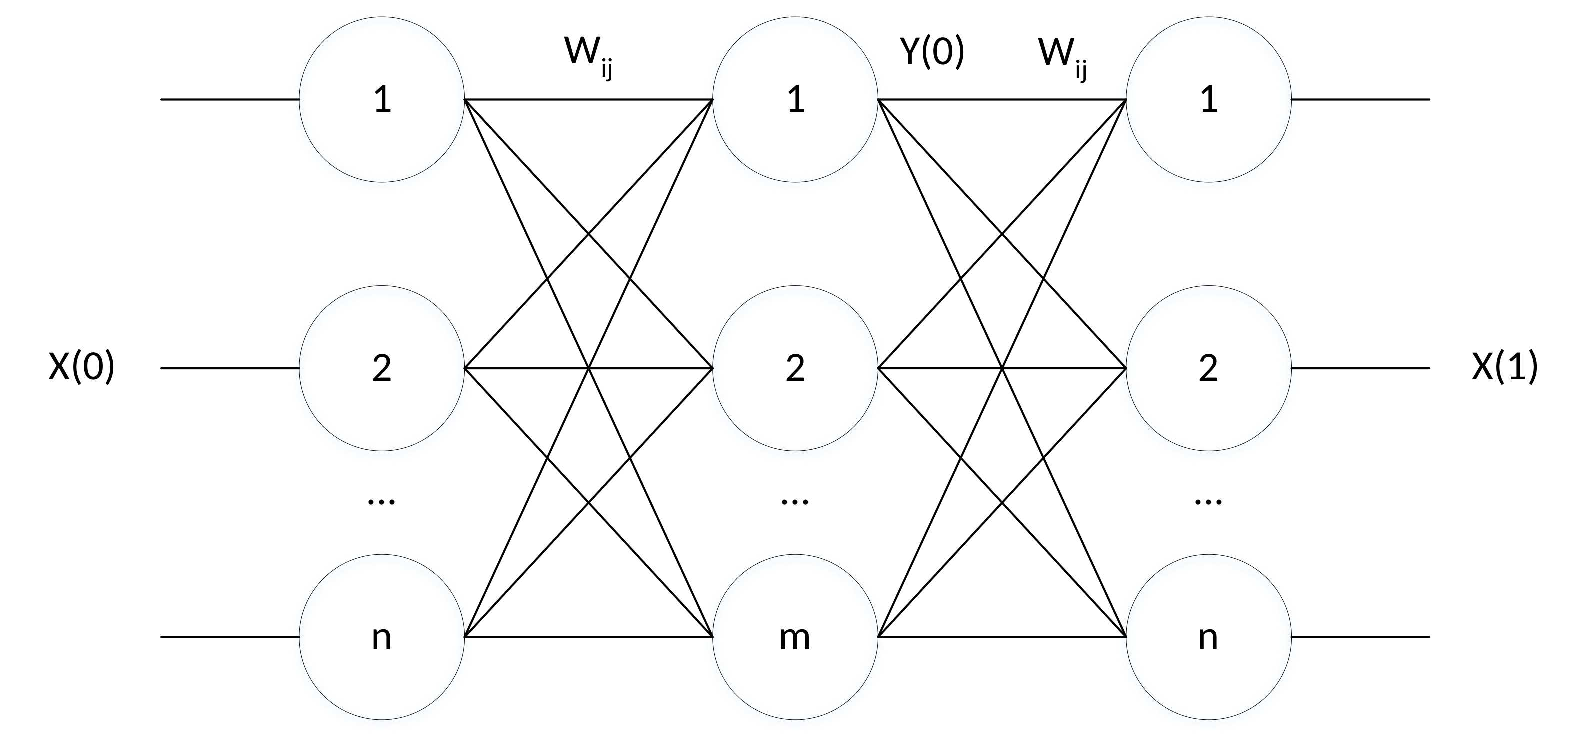
\includegraphics[width=0.9\textwidth]{man-source/images/ch2/pic2-1.pdf}
  \caption{Развернутое представление RBM}
  \label{fig:pic2_1}
\end{figure}

Представим сэмплирование Гиббса, используя развернутое представление RBM (рисунок~\ref{fig:pic2_2}).

\begin{figure}[H]
  \centering
  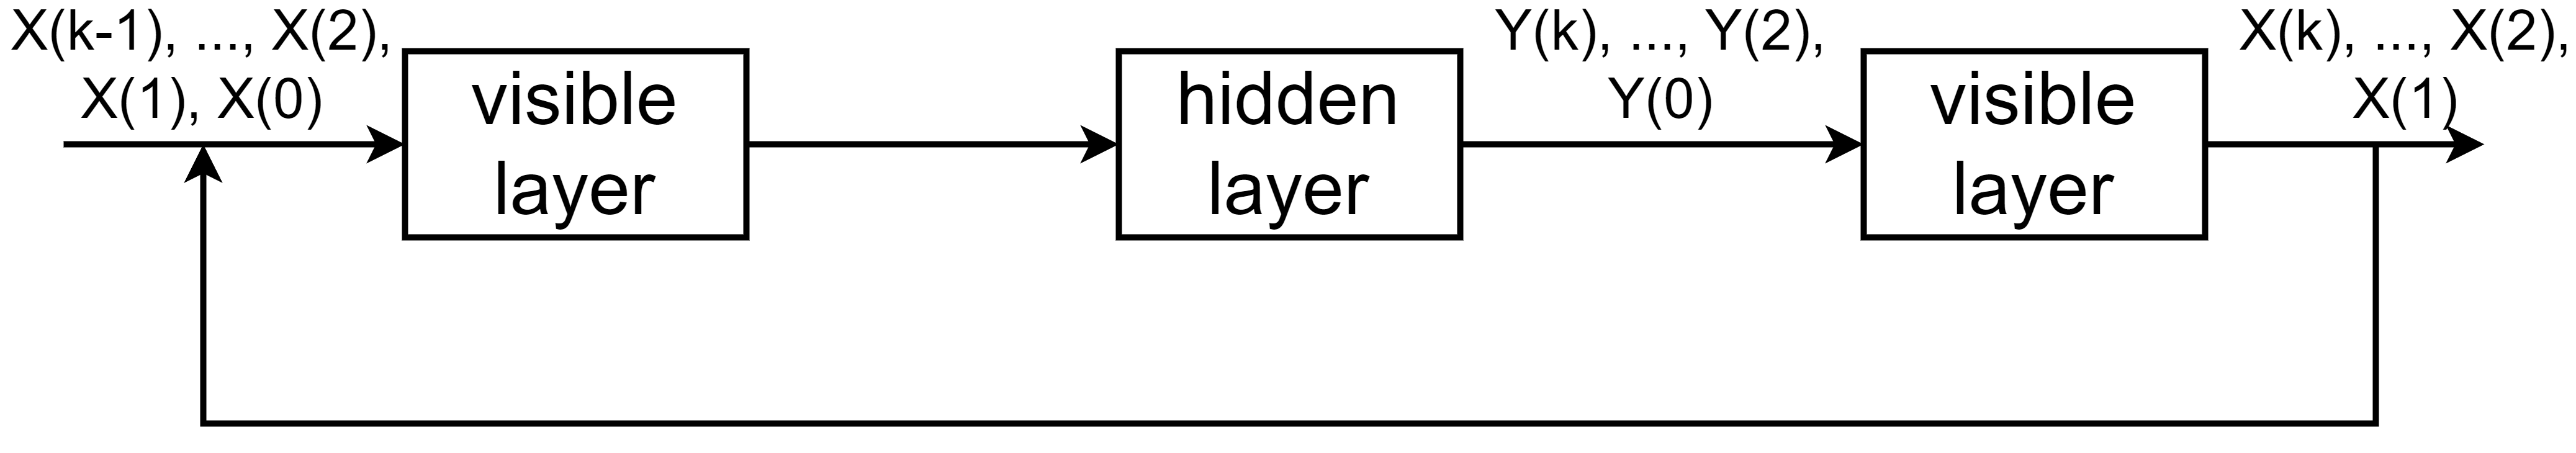
\includegraphics[width=\textwidth]{man-source/images/ch2/pic2-2.png}
  \caption{Сэмплирование Гиббса}
  \label{fig:pic2_2}
\end{figure}

Сэмплирование Гиббса заключается в следующей процедуре. Пусть $x(0)$ -- входной вектор, который поступает на видимый слой в момент времени $t=0$. Тогда выходные значения нейронов скрытого слоя будут определяться следующим образом:

\begin{equation}
    y_j(0)=F(S_j(0)),
\end{equation}

\begin{equation}
    S_j(0)=\sum_i w_{ij}x_i(0)+T_j.
\end{equation}

Инверсный (последний) слой  реконструирует входной вектор на основе данных со скрытого слоя и текущего значения настраиваемых параметров (порогов видимого слоя и матрицы весов). В результате получается восстановленный вектор $x(1)$ в момент времени $t=1$:

\begin{equation}
    x_i(1)=F(S_i(1)),
\end{equation}

\begin{equation}
    S_i(1)=\sum_j w_{ij}y_j(0)+T_i.
\end{equation}

Затем вектор $x(1)$ поступает на видимый слой, и вычисляются выходные значения нейронов скрытого слоя: 

\begin{equation}
    y_j(1)=F(S_j(1)),
\end{equation}

\begin{equation}
    S_j(1)=\sum_i w_{ij}x_i(1)+T_j.
\end{equation}

Продолжая данный процесс, можно получить на шаге k следующие выражения:

\begin{equation*}		
    y_j(k)=F(S_j(k)),\ S_j(k)=\sum_i w_{ij}x_i(k)+T_j,
\end{equation*}

\begin{equation*}		
    x_i(k)=F(S_i(k)),\ S_i(k)=\sum_j w_{ij}y_j(k-1)+T_i.
\end{equation*}

\section{Вывод правил предобучения} 

Хинтоном была предложена энергетическая модель, базирующаяся на идее максимизации функции правдоподобия распределения входных данных $P(x)$. Вывод классических правил обучения был приведен в главе I. Основываясь на идее использования ограниченной машины Больцмана в качестве вспомогательной модели для проведения предобучения, было предложено использование двух разных критериев для ее обучения \cite{4-A}. Первый критерий основывается на минимизации среднеквадратичной ошибки (MSE), а второй -- на минимизации кросс-энтропийной функции ошибки.

Покажем, что применение различных критериев минимизации позволяет, тем не менее, получить одинаковые правила обучения.

\subsection{Критерий MSE}

В случае использования в качестве критерия обучения MSE основной целью обучения ограниченной машины Больцмана является минимизация суммарной среднеквадратичной ошибки реконструкции данных на скрытом и видимом (восстанавливающем) слое, которая в случае CD-k определяется следующим образом:	

\begin{equation*}	
    E_s(k)=\frac{1}{2L}\Bigg(\sum_{l=1}^L\sum_{j=1}^m\sum_{p=1}^k (y_j^l(p)-y_j^l(p-1))^2+\sum_{l=1}^L\sum_{i=1}^n\sum_{p=1}^k (x_i^l(p)-x_i^l(p-1))^2\Bigg),
\end{equation*}
где \textit{k} определяет параметр процедуры сэмплирования Гиббса,\\
\textit{n} -- количество нейронов в видимом слое,\\
\textit{m} -- количество нейронов в скрытом слое,\\
\textit{L} -- размерность обучающей выборки.

В случае CD-1  суммарная среднеквадратичная ошибка:

\begin{equation}
    E_s(1)=\frac{1}{2L}\Bigg(\sum_{l=1}^L\sum_{j=1}^m (y_j^l(1)-y_j^l(0))^2+\sum_{l=1}^L\sum_{i=1}^n (x_i^l(1)-x_i^l(0))^2\Bigg).
\end{equation}

Как следует из приведенных выше выражений, ошибка состоит из двух частей: ошибки восстановления информации на видимом и скрытом слоях, то есть может быть представлена в следующем виде:
\begin{equation}
	\label{mse_rbm_criteria}
	E_s(k) = E_h(k) + E_v(k),
\end{equation}
где

\begin{equation}
	E_h(k) = \frac{1}{2L}\sum_{l=1}^L\sum_{j=1}^m\sum_{p=1}^k (y_j^l(p)-y_j^l(p-1))^2,
\end{equation}

\begin{equation}
	E_v(k) = \frac{1}{2L}\sum_{l=1}^L\sum_{i=1}^n\sum_{p=1}^k (x_i^l(p)-x_i^l(p-1))^2.
\end{equation}

Найдем правила обучения, соответствующие критерию \ref{mse_rbm_criteria} и докажем их эквивалентность классическим правилам обучения RBM при выполнении некоторых специальных условий.

\textbf{Теорема 1}. Максимизация функции правдоподобия распределения данных $P(x)$ в пространстве синаптических связей ограниченной машины Больцмана эквивалентна минимизации суммарной квадратичной ошибки сети в том же пространстве при использовании линейных нейронов.

\textbf{Доказательство}: Рассмотрим последовательное обучение RBM, когда модификация синаптических связей происходит после подачи каждого входного образа на сеть (онлайн-обучение). В соответствии с методом градиентного спуска для минимизации суммарной квадратичной ошибки сети, синаптические связи должны изменяться следующим образом:	

\begin{equation}
w_{ij}(t+1)=w_{ij}(t)-\alpha\frac{\partial E}{\partial w_{ij}(t)},
\end{equation}		

\begin{equation}
T_{i}(t+1)=T_{i}(t)-\alpha\frac{\partial E}{\partial T_{i}(t)},
\end{equation}		

\begin{equation}
T_{j}(t+1)=T_{j}(t)-\alpha\frac{\partial E}{\partial T_{j}(t)}.
\end{equation}

В случае CD-k квадратичная ошибка $E$ для одного образа:

\begin{equation*}
E=\frac{1}{2}\sum_{j=1}^m\sum_{p=1}^k (y_j(p)-y_j(p-1))^2+\frac{1}{2}\sum_{i=1}^n\sum_{p=1}^k (x_i(p)-x_i(p-1))^2.
\end{equation*}

Тогда
\begin{multline*}
    \frac{\partial E}{\partial w_{ij}}=\frac{\partial E}{\partial y_j(p)}\frac{\partial y_j(p)}{\partial S_j(p)}\frac{\partial S_j(p)}{\partial w_{ij}}+\frac{\partial E}{\partial x_i(p)}\frac{\partial x_i(p)}{\partial S_i(p)}\frac{\partial S_i(p)}{\partial w_{ij}}=\\=\sum_{p=1}^k (y_j(p)-y_j(p-1))x_i(p)F'(S_j(p))+\\+\sum_{p=1}^k (x_i(p)-x_i(p-1))y_j(p-1)F'(S_i(p)).
\end{multline*}

Если ограниченная машина Больцмана использует линейные нейроны с линейной функцией активации, то

\begin{equation*}
    \frac{\partial S_i(p)}{\partial w_{ij}}=F'(S_i(p))=\frac{\partial S_j(p)}{\partial w_{ij}}=F'(S_j(p))=1.
\end{equation*}

Тогда

\begin{equation*}
    \frac{\partial E}{\partial w_{ij}}=\sum_{p=1}^k (y_j(p)x_i(p)-y_j(p-1)x_i(p-1))=y_j(k)x_i(k)-y_j(0)x_i(0).
\end{equation*}

В результате можно получить CD-k правило обучения RBM:

\begin{equation*}
    w_{ij}(t+1)=w_{ij}(t)+\alpha(x_i(0)y_j(0)-x_i(k)y_j(k)).
\end{equation*}

Аналогичным образом для пороговых значений:

\begin{equation*}
\begin{aligned}
    T_{j}(t+1)=T_{j}(t)+\alpha(y_j(0)-y_j(k)),\\
    T_{i}(t+1)=T_{i}(t)+\alpha(x_i(0)-x_i(k)).
\end{aligned}
\end{equation*}

Как видно последние выражения совпадают с классическим правилом обучения ограниченной машины Больцмана для CD-k. Отсюда следует, что для линейной RBM максимизация функции правдоподобия распределения данных $P(x)$ эквивалентна минимизации суммарной квадратичной ошибки сети. Теорема доказана.

\textbf{Следствие 1.1}. Линейная ограниченная машина Больцмана c точки зрения обучения эквивалентна автоассоциативной нейронной сети при использовании в ней при обучении сэмплирования Гиббса.

\textbf{Следствие 1.2}. Для нелинейной ограниченной машины Больцмана правило модификации синаптических связей в случае CD-k будет следующим:
\begin{multline*}
    w_{ij}(t+1)=w_{ij}(t)-\\-\alpha\Bigg(\sum_{p=1}^k (y_j(p)-y_j(p-1))x_i(p)F'(S_j(p))+(x_i(p)-x_i(p-1))y_j(p-1)F'(S_i(p))\Bigg),
\end{multline*}

\begin{equation*}
\begin{aligned}
    T_i(t+1)=T_i(t)-\alpha\left(\sum_{p=1}^k (x_i(p)-x_i(p-1))F'(S_i(p))\right),\\
    T_j(t+1)=T_j(t)-\alpha\left(\sum_{p=1}^k (y_j(p)-y_j(p-1))F'(S_j(p))\right).
\end{aligned}
\end{equation*}

\textbf{Следствие 1.3}. Для нелинейной ограниченной машины Больцмана правило модификации синаптических связей в случае CD-1 будет следующим:	
\begin{equation*}
    w_{ij}(t+1)=w_{ij}(t)-\alpha((y_j(1)-y_j(0))F'(S_j(1))x_i(1)+(x_i(1)-x_i(0))F'(S_i(1))y_j(0)),
\end{equation*}

\begin{equation*}
    T_i(t+1)=T_i(t)-\alpha(x_i(1)-x_i(0))F'(S_i(1)),
\end{equation*}

\begin{equation*}
    T_j(t+1)=T_j(t)-\alpha(y_j(1)-y_j(0))F'(S_j(1)).  
\end{equation*}

При использовании группового обучения (batch learning), метод градиентного спуска примет следующий вид:

\begin{equation}
    w_{ij}(t+1)=w_{ij}(t)-\alpha\frac{\partial E_s}{\partial w_{ij}(t)},
\end{equation}

\begin{equation}
    T_{i}(t+1)=T_{i}(t)-\alpha\frac{\partial E_s}{\partial T_{i}(t)},
\end{equation}

\begin{equation}
    T_{j}(t+1)=T_{j}(t)-\alpha\frac{\partial E_s}{\partial T_{j}(t)}.
\end{equation}

\textbf{Теорема 2}. При использовании  CD-k для нелинейной ограниченной машины Больцмана в случае группового обучения правило модификации синаптических связей определяется на основе следующих выражений:
\begin{multline*}
    w_{ij}(t+1)=w_{ij}(t)-\\-\frac{\alpha}{L}\Bigg(\sum_{l=1}^L\sum_{p=1}^k (y_j^l(p)-y_j^l(p-1))x_i^l(p)F'(S_j^l(p))+(x_i^l(p)-x_i^l(p-1))y_j^l(p-1)F'(S_i^l(p))\Bigg),
\end{multline*}

\begin{equation*}
    T_{i}(t+1)=T_{i}(t)-\frac{\alpha}{L}\left(\sum_{l=1}^L\sum_{p=1}^k (x_i^l(p)-x_i^l(p-1))F'(S_i^l(p))\right),
\end{equation*}

\begin{equation*}
    T_{j}(t+1)=T_{j}(t)-\frac{\alpha}{L}\left(\sum_{l=1}^L\sum_{p=1}^k (y_j^l(p)-y_j^l(p-1))F'(S_j^l(p))\right).
\end{equation*}

Процесс доказательства данной теоремы является аналогичным доказательству теоремы 1.

\textbf{Следствие 2.1}. При использовании  CD-1 для нелинейной ограниченной машины Больцмана в случае группового обучения правило модификации синаптических связей определяется на основе следующих выражений:

\begin{multline*}
    w_{ij}(t+1)=w_{ij}(t)-\\-\frac{\alpha}{L}\left(\sum_{l=1}^L (y_j^l(1)-y_j^l(0))x_i^l(1)F'(S_j^l(1))+(x_i^l(1)-x_i^l(0))y_j^l(0)F'(S_i^l(1))\Bigg)\right.,
\end{multline*}

\begin{equation*}
    T_i(t+1)=T_i(t)-\frac{\alpha}{L}\left(\sum_{l=1}^L (x_i^l(1)-x_i^l(0))F'(S_i^l(1))\right),
\end{equation*}

\begin{equation*}
    T_j(t+1)=T_j(t)-\frac{\alpha}{L}\left(\sum_{l=1}^L (y_j^l(1)-y_j^l(0))F'(S_j^l(1))\right).
\end{equation*}

\textbf{Следствие 2.2}. При использовании  CD-k для линейной ограниченной машины Больцмана в случае группового обучения правило модификации синаптических связей определяется на основе следующих выражений:

\begin{equation*}
    w_{ij}(t+1)=w_{ij}(t)+\frac{\alpha}{L}\sum_{l=1}^L (x_i^l(0)y_j^l(0)-x_i^l(k)y_j^l(k)),
\end{equation*}

\begin{equation*}
    T_{i}(t+1)=T_{i}(t)+\frac{\alpha}{L}\sum_{l=1}^L (x_i^l(0)-x_i^l(k)),
\end{equation*}

\begin{equation*}
    T_{j}(t+1)=T_{j}(t)+\frac{\alpha}{L}\sum_{l=1}^L (y_j^l(0)-y_j^l(k)).
\end{equation*}

\textbf{Следствие 2.3}. При использовании  CD-1 для линейной ограниченной машины Больцмана в случае группового обучения правило модификации синаптических связей определяется на основе следующих выражений:

\begin{equation*}
    w_{ij}(t+1)=w_{ij}(t)+\frac{\alpha}{L}\sum_{l=1}^L (x_i^l(0)y_j^l(0)-x_i^l(1)y_j^l(1)),
\end{equation*}

\begin{equation*}
    T_{i}(t+1)=T_{i}(t)+\frac{\alpha}{L}\sum_{l=1}^L (x_i^l(0)-x_i^l(1)),
\end{equation*}

\begin{equation*}
    T_{j}(t+1)=T_{j}(t)+\frac{\alpha}{L}\sum_{l=1}^L (y_j^l(0)-y_j^l(1)).
\end{equation*}

Таким образом, получены правила обучения для ограниченной машины Больцмана, которые базируются на минимизации квадратичной ошибки восстановления информации на видимом и скрытом слоях.  Предложенный метод позволяет учитывать нелинейную природу нейронных элементов. Показано, что классические выражения для обучения ограниченной машины являются частным случаем предложенного метода. Доказана теорема об эквивалентности максимизации функции правдоподобия распределения входных данных $P(x)$ и минимизации суммарной квадратичной ошибки сети в одном и том же пространстве синаптических связей для линейной ограниченной машины Больцмана. 

\subsection{Критерий СЕ}

В случае CD-k кросс-энтропийная функция ошибки для видимого слоя определяется следующим образом:

\begin{equation*}
	CE_v(k) = -\frac{1}{L}\sum_{l=1}^L \sum_{p=1}^k \sum_{i=1}^n x_i^l(p-1)\log(x_i^l(p))+(1-x_i^l(p-1)\log(1-x_i^l(p)),
\end{equation*}
где $L$ -- размер обучающей выборки,\\
$k$ -- параметр процедуры сэмплирования,\\
$n$ -- количество нейронов на видимом слое.

Аналогично для скрытого слоя:

\begin{equation*}
	CE_h(k) = -\frac{1}{L}\sum_{l=1}^L \sum_{p=1}^k \sum_{j=1}^m y_j^l(p-1)\log(y_j^l(p))+(1-y_j^l(p-1)\log(1-y_j^l(p)),
\end{equation*}
где $m$ -- количество нейронов на скрытом слое.

Общая функция определяется как сумма кросс-энтропийных функций ошибки видимого и скрытого слоев:

\begin{equation}
	CE_s(k) = CE_h(k)+CE_v(k).
\end{equation}

Докажем следующую теорему.

\textbf{Теорема 3}. Максимизация функции правдоподобия распределения входных данных $P(x)$ эквивалентна минимизации кросс-энтропийной целевой функции $CE_s(k)$ в одном и том же пространстве синаптических весов ограниченной машины Больцмана (случай $k=1$).

\textbf{Доказательство}. В случае CD-1 кросс-энтропийная функция для одного обучающего примера будет иметь следующий вид:

\begin{multline}
	CE(1) = -\sum_{i=1}^n (x_i(0)\log(x_i(1))+(1-x_i(0))\log(1-x_i(1)))-\\-\sum_{j=1}^m ( y_j(0)\log(y_j(1))+(1-y_j(0))\log(1-y_j(1))) = \\ = CE_v(1)+CE_h(1).
\end{multline}

Найдем частные производные кросс-энтропийной функции по весовым элементам. Получим

\begin{equation*}
	\frac{\partial CE(1)}{\partial w_{ij}} = \frac{\partial CE_v(1)}{\partial w_{ij}} + \frac{\partial CE_h(1)}{\partial w_{ij}}.
\end{equation*}

Тогда

\begin{multline*}
	\frac{\partial CE_v(1)}{\partial w_{ij}} = -\frac{x_i(0)}{x_i(1)}x_i(1)(1-x_i(1))y_j(0)+\frac{1-x_i(0)}{1-x_i(1)}x_i(1)(1-x_i(1))y_j(0) = \\ = -x_i(0)(1-x_i(1))y_j(0)+(1-x_i(0))x_i(1)y_j(0)=\\=-x_i(0)y_j(0)+x_i(0)x_i(1)y_j(0)+x_i(1)y_j(0)-x_i(0)x_i(1)y_j(0)=\\=-x_i(0)y_j(0)+x_i(1)y_j(0) 
\end{multline*}

и

\begin{multline*}
	\frac{\partial CE_h(1)}{\partial w_{ij}} = -y_j(0)(1-y_j(1))x_i(1)+(1-y_j(0))y_j(1)x_i(1) = \\ = -y_j(0)x_i(0)+y_j(0)y_j(1)x_i(1)+y_j(1)x_i(1)-y_j(0)y_j(1)x_i(1) = \\ = -y_j(0)x_i(1)+y_j(1)x_i(1). 
\end{multline*}

Окончательно получим

\begin{multline*}
	\frac{\partial CE(1)}{\partial w_{ij}} = \frac{\partial CE_v(1)}{\partial w_{ij}} + \frac{\partial CE_h(1)}{\partial w_{ij}} = \\ = -x_i(0)y_j(0)+x_i(1)y_j(0) -y_j(0)x_i(1)+y_j(1)x_i(1) = x_i(1)y_j(1) - x_i(0)y_j(0).
\end{multline*}

Аналогично, для пороговых элементов имеем:

\begin{multline*}
	\frac{\partial CE(1)}{\partial T_i} = \frac{\partial CE_v(1)}{\partial T_i} = -\frac{x_i(0)}{x_i(1)}x_i(1)(1-x_i(1))+\frac{1-x_i(0)}{1-x_i(1)}x_i(1)(1-x_i(1)) = \\ = -x_i(0) + x_i(0)x_i(1)+x_i(1)-x_i(0)x_i(1) = x_i(1)-x_i(0);
\end{multline*}

\begin{multline*}
	\frac{\partial CE(1)}{\partial T_j} = \frac{\partial CE_h(1)}{\partial T_j} = -y_j(0)(1-y_j(1)) + (1-y_j(0))y_j(1) = \\ = -y_j(0) + y_j(0)y_j(1) + y_j(1) - y_j(0)y_j(1) = y_j(1) - y_j(0).
\end{multline*}

Теорема доказана. 

Рассматривая более общий случай CD-k, можно доказать следующую теорему.

\textbf{Теорема 4}. Максимизация функции правдоподобия распределения входных данных $P(x)$ эквивалентна минимизации кросс-энтропийной целевой функции $CE_s(k)$ в одном и том же пространстве синаптических весов ограниченной машины Больцмана (случай произвольного $k$).

\textbf{Доказательство}. В случае CD-k кросс-энтропийная функция для одного обучающего примера будет иметь следующий вид:

\begin{multline}
	CE_s(k) = -\sum_{p=1}^k \sum_{i=1}^n (x_i(p-1)\log(x_i(p)) + (1-x_i(p-1))\log(1-x_i(p)))-\\-\sum_{p=1}^k \sum_{j=1}^m (y_j(p-1)\log (y_j(p))+(1-y_j(p-1))\log(1-y_j(p))) = \\ = CE_v(k) + CE_h(k).
\end{multline}

Как и в случае CD-1 находим соответствующие частные производные по весовым и пороговым элементам. Имеем:

\begin{equation*}
	\frac{\partial CE_s(k)}{\partial w_{ij}}= \frac{\partial CE_v(k)}{\partial w_{ij}} + \frac{\partial CE_h(k)}{\partial w_{ij}}.
\end{equation*}

Причем

\begin{multline*}
	\frac{\partial CE_v(k)}{\partial w_{ij}} = \\ = -\sum_{p=1}^k (x_i(p-1)(1-x_i(p))y_j(p-1)-(1-x_i(p-1))x_i(p)y_j(p-1))=\\=-\sum_{p=1}^k (x_i(p-1)y_j(p-1)-x_i(p-1)x_i(p)y_j(p-1)-\\-x_i(p)y_j(p-1)+x_i(p-1)x_i(p)y_j(p-1)) = \\ = \sum_{p=1}^{k} (x_i(p)y_j(p-1)-x_i(p-1)y_j(p-1))
\end{multline*}

и

\begin{multline*}
	\frac{\partial CE_h(k)}{\partial w_{ij}} = \\ = -\sum_{p=1}^k (y_j(p-1)(1-y_j(p))x_i(p)-(1-y_j(p-1))y_j(p)x_i(p)) = \\ = -\sum_{p=1}^{k} (y_j(p-1)x_i(p)-y_j(p-1)y_j(p)x_i(p)-\\-y_j(p)x_i(p)+y_j(p-1)y_j(p)x_i(p)) = \\ = \sum_{p=1}^{k} (x_i(p)y_j(p)-x_i(p)y_j(p-1)).
\end{multline*}

А значит

\begin{multline*}
	\frac{\partial CE_s(k)}{\partial w_{ij}} = \sum_{p=1}^{k}(y_j(p)x_i(p)-x_i(p-1)y_j(p-1)) = \\ = y_j(1)x_i(1)-x_i(0)y_j(0)+x_i(2)y_j(2)-x_i(1)y_j(1)+\dots+\\+x_i(k)y_j(k)-x_i(k-1)y_j(k-1)=\\=x_i(k)y_j(k)-x_i(0)y_j(0).
\end{multline*}

Аналогично для пороговых элементов:

\begin{multline*}
	\frac{\partial CE_s(k)}{\partial T_i} = \frac{\partial CE_v(k)}{\partial T_i} =\\= -\sum_{p=1}^k (x_i(p-1)(1-x_i(p))-(1-x_i(p-1))x_i(p)) =\\= \sum_{p=1}^k (x_i(p) - x_i(p-1)) = x_i(1)-x_i(0)+x_i(2) - x_i(1) +\dots+x_i(k)-x_i(k-1) =\\= x_i(k)-x_i(0);
\end{multline*}

\begin{multline*}
	\frac{\partial CE_s(k)}{\partial T_j} = \frac{\partial CE_h(k)}{\partial T_j} =\\= -\sum_{p=1}^k (y_j(p-1)(1-y_j(p))-(1-y_j(p-1))y_j(p)) =\\= \sum_{p=1}^k (y_j(p) - y_j(p-1)) = y_j(1)-y_j(0)+y_j(2) - y_j(1) +\dots+y_j(k)-y_j(k-1) =\\= y_j(k)-y_j(0).
\end{multline*}

Теорема доказана.

Из доказанных теорем 3 и 4 следует, что правила обучения ограниченной машины Больцмана могут быть получены более простым путем, чем при использовании традиционного подхода, основанного на применении функции энергии. Произведя минимизацию кросс-энтропийной функции и применяя простые итерации сэмплирования Гиббса, мы получили классические линейные правила обучения RBM.

Таким образом, на основании доказанных теорем 1-4 можно сформулировать общую теорему.

\textbf{Теорема 5}. Максимизация функции правдоподобия распределения входных данных $P(x)$ эквивалентна минимизации кросс-энтропийной функции и специальному случаю минимизации среднеквадратичной ошибки в одном и том же пространстве синаптических весов ограниченной машины Больцмана:

\begin{equation}
	\max(\ln P(x)) = \min(CE_s) = \min(E_s).
\end{equation}

Теорема 5 обобщает предыдущие результаты. Как следует из этой теоремы, использование различных критериев обучения приводит к тем же самым правилам. Поэтому сущность неконтролируемого обучения для ограниченной машины Больцмана одинакова, даже если используются различные целевые функции. Максимизация функции правдоподобия и минимизация кросс-энтропийной функции ошибки приводит к линейному представлению нейронных элементов в терминах минимизации функции MSE. Необходимо отметить, что, применяя критерий MSE, мы учитываем также нелинейное представление нейронных элементов. Таким образом, очевидное преимущество в использовании MSE в качестве функции ошибок перед применением функции максимального правдоподобия и кросс-энтропийной функции в том, что при использовании MSE могут быть получены как линейные, так и нелинейные правила обучения.

В дальнейшем для идентификации предлагаемого подхода будем использовать аббревиатуру REBA (Reconstruction Error-Based Approach). Классический метод будем называть C-RBM (Classic Restricted Boltzmann Machine Training).

\section{Предобучение сверточных слоев}

Выполнение предобучения сверточных слоев имеет особое значение при решении задач компьютерного зрения в силу эффективности таких слоев при обработке визуальной информации, представленной с помощью отдельных изображений и видео.

Отметим, что преобразования, выполняемые над сверточными слоями при обучении, идентичны преобразованиям для полносвязных слоев. 
Отличие заключается в операции <<развертки>> (deconvolution), которая используется на этапе предобучения при реконструкции активности видимых нейронов и на этапе тонкой настройки для метода обратного распространения при вычислении ошибок на скрытых слоях сети. Эта операция применяется в сверточных нейронных сетях для повышения частоты дискретизации.
Рассмотрим визуальное представление операции свертки для случая карт 3Х3 и 2Х2 (рисунок \ref{fig:convolution}).

\begin{figure}[H]
  \centering
  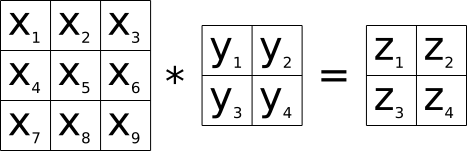
\includegraphics[width=0.5\textwidth]{man-source/images/ch2/pic2-4.png}
  \caption{Операция свертки}
  \label{fig:convolution}
\end{figure}

Сверточный слой с одним ядром может быть представлен в виде разряженного слоя, а операция <<развертки>> -- слоем, полученным применением симметричного преобразования относительно разряженного. При этом полученная сеть представляет собой автоэнкодер с симметричными связями относительно скрытого слоя (рисунок \ref{fig:convolution_autoencoder}).

На основании данного представления могут быть получены формулы для выполнения <<развертки>>:

\begin{equation*}
	x'_1 = z_1y_1		
	\end{equation*}
	\begin{equation*}
	x'_2 = z_1y_2+z_2y_1
	\end{equation*}
	\begin{equation*}
	x'_3 = z_2y_2
	\end{equation*}
	\begin{equation*}
	x'_4 = z_1y_3 + z_3y_1
	\end{equation*}
	\begin{equation*}
	x'_5 = z_1y_4 + z_2y_3 + z_3y_2 + z_4y_1
	\end{equation*}
	\begin{equation*}
	x'_6 = z_2y_4 + z_4y_2
	\end{equation*}
	\begin{equation*}
	x'_7 = z_3y_3
	\end{equation*}
	\begin{equation*}
	x'_8 = z_3y_4 + z_4y_3
	\end{equation*}		
	\begin{equation*}
	x'_9 = z_4y_4
	\end{equation*}	

\begin{figure}[H]
  \centering
  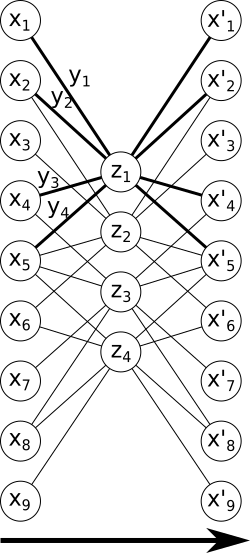
\includegraphics[width=0.4\textwidth]{man-source/images/ch2/pic2-5.png}
  \caption{Разряженный автоэнкодер операции свертки}
  \label{fig:convolution_autoencoder}
\end{figure}

Сама операция <<развертки>> представлена на рисунке \ref{fig:deconvolution}.

\begin{figure}[H]
  \centering
  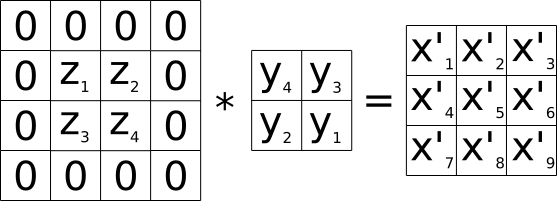
\includegraphics[width=0.6\textwidth]{man-source/images/ch2/pic2-6.png}
  \caption{Операция <<развертки>>}
  \label{fig:deconvolution}
\end{figure}

Введя операции матричного поворота на 180 градусов и заполнения нулями границ матрицы (padding), можно получить следующие общие формулы для выполнения <<развертки>> (рисунок \ref{fig:deconvolution_formula}).

\begin{figure}[H]
  \centering
  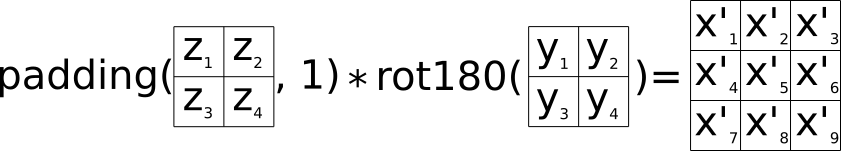
\includegraphics[width=0.9\textwidth]{man-source/images/ch2/pic2-9.png}
  \caption{Формула <<развертки>>}
  \label{fig:deconvolution_formula}
\end{figure}

Введем условное обозначение для операции <<развертки>> -- $\circledast$.

Применяя полученную формулу для выполнения <<развертки>>, можно осуществлять процедуру CD на сверточных слоях ГНС, которые в этом случае рассматриваются как сверточные ограниченные машины Больцмана (CRBM). 

Рассмотрим формулы для получения необходимых карт признаков для расчета градиента изменения параметров слоя в случае использования процедуры CD-1: 

\begin{equation*}
    y_j(0) = F(x_i(0) * w_{ij} + T_j),
\end{equation*}

\begin{equation*}
    x_i(1) = F(y_j(0) \circledast w_{ij} + T_i),
\end{equation*}

\begin{equation*}
    y_j(1) = F(x_i(1) * w_{ij} + T_j),
\end{equation*}
где $w_{ij}$ -- $i$-тый компонент $j$-того ядра свертки,\\
$x_i(0)$ -- $i$-тый компонент входной карты признаков,\\
$T_j$ -- пороговый элемент $j$-того нейрона скрытого слоя,\\
$y_j(0)$ -- $j$-тый компонент выходной карты признаков,\\
$x_i(1)$ -- $i$-тый компонент реконструированной входной карты признаков,\\
$T_i$ -- пороговый элемент $i$-того нейрона видимого слоя,\\
$y_j(1)$ -- $j$-тый компонент реконструированной выходной карты признаков.

Классические правила обучения RBM могут быть переформулированы для случая CRBM (CD-1, последовательное обучение): 

\begin{equation*}
		w_{ij}(t+1)=w_{ij}(t)+\alpha(x_i(0) * y_j(0)-x_i(1) * y_j(1)),
\end{equation*} 

\begin{equation*}	
		T_i(t+1)=T_i(t)+\alpha(x_i(0)-x_i(1)),
\end{equation*} 

\begin{equation*}		
		T_j(t+1)=T_j(t)+\alpha(y_j(0)-y_j(1)).
\end{equation*}
% где $\circledast$ обозначает операцию свертки.

В соответствии с предлагаемым методом, правила обучения могут быть переформулированы следующим образом (CD-1, последовательное обучение):

\begin{multline*}
    w_{ij}(t+1)=w_{ij}(t)-\alpha((y_j(1)-y_j(0))F'(S_j(1)) * x_i(1)+\\(x_i(1)-x_i(0))F'(S_i(1)) * y_j(0)),    
\end{multline*}
\begin{equation*}
    T_i(t+1)=T_i(t)-\alpha(x_i(1)-x_i(0))F'(S_i(1)),
\end{equation*}
\begin{equation*}
    T_j(t+1)=T_j(t)-\alpha(y_j(1)-y_j(0))F'(S_j(1)).  
\end{equation*}

Аналогичным образом могут быть получены правила для CD-\textit{k} случая процедуры обучения и группового случая.

Таким образом, для глубокой сверточной нейронной сети, содержащей слои разных типов (полносвязные и сверточные) возможно сочетание нескольких вариантов обучения -- с представлением в виде CRBM (для сверточных слоев) и в виде RBM (для полносвязных).  

\section{Метод редуцирования параметров}
Известно, что полносвязные нейронные сети обладают определенной степенью избыточности. Полносвязный слой в сравнении со сверточным содержит большее количество настраиваемых параметров, однако в задачах компьютерного зрения сверточные нейронные сети показывают существенно лучшие результаты по обобщающей способности, чем полносвязные. Таким образом, очевидно, что в полносвязных сетях при большем количестве настраиваемых параметров, они используются менее оптимально. Можно предположить, что указанные <<избыточные>> параметры могут быть исключены без существенного ухудшения эффективности работы модели. Важный вопрос, возникающий при выполнении такой операции редуцирования, касается самого алгоритма отсеивания малоинформативных параметров.

К основным методам компрессии (сжатия) нейросетевых моделей на настоящий момент относятся:
\begin{easylistNum}
	& прунинг -- pruning (\cite{wang2019pruning}, \cite{xu2020});
	& квантизация -- quantization \cite{hubara2016quantized};
	& дистилляция -- distillation \cite{Hinton2015DistillingTK};
	& матричная факторизация низкого ранга -- low-rank matrix factorization \cite{Sainath2013}.
\end{easylistNum}

\textit{Прунинг} позволяет удалить часть связей и нейронов (в зависимости от выполняемой техники редуцирования), что уменьшает структурную избыточность <<тяжелых>> глубоких нейросетевых моделей.
По типу выполняемой техники прунинга выделяют:

\begin{easylist}
	& прунинг связей;
	& прунинг нейронов или фильтров (в зависимости от типа слоя -- полносвязного или сверточного);
	& прунинг слоев.
\end{easylist}

\textit{Квантизация} используется для физического уменьшения памяти, занимаемой моделью. В этом подходе осуществляется редуцирование типа данных, используемого для хранения параметров нейросетевой модели (например, осуществляется переход от 32-битного к 16-битному или 8-битному представлению типа).

\textit{Дистилляция} основывается на возможности использования более <<тяжелых>> моделей для обучения моделей меньшего размера. В этом случае обученная модель-учитель генерирует примеры, которые используются для обучения модели-ученика. Размер такой модели-ученика может быть существенно меньше первоначальной сети. По разновидностям выделяют следующие типы дистилляции:

\begin{easylist}
	& офлайн-дистилляция (применяется последовательное обучение модели-учителя, затем -- модели-ученика);
	& онлайн-дистилляция (применяется одновременное обучение модели-учителя и модели-ученика);
	& самодистилляция (в качестве модели-учителя и модели-ученика выступает одна модель).
\end{easylist}

Наконец, \textit{матричная факторизация низкого ранга} позволяет осуществить декомпозицию матрицы весовых коэффициентов большого размера на совокупность матриц меньшего размера. Применение данного подхода помогает уменьшить память, занимаемую моделями и ускорить время работы модели. К недостаткам метода относят его вычислительную сложность.
% Редуцирование параметров нейросетевой модели позволяет добиться уменьшения количества настраиваемых параметров, что может быть актуальным при применении нейронных сетей на устройствах с ограниченными аппаратными возможностями (одноплатные компьютеры, мобильные телефоны и т.д.). Применение при этом специальных методик для хранения разряженных матриц позволяет ускорить работу архитектуры. Важно, чтобы при этом сеть сохраняла свою обобщающую способность.

Предлагаемый алгоритм редуцирования связей НС основывается на прунинге, но имеет модификацию, которая заключается в наличии этапа неконтролируемого предобучения на основе RBM.

Рассмотрим подход для редуцирования связей полносвязной нейронной сети, основанный на использовании предобучения. Первый и четвертый этапы данной процедуры аналогичны этапам выполнения предобучения типа II, описанного в главе I. В ходе выполнения дополнительных этапов 2 и 3 формируются разряженные связи между входными и выходными нейронными элементами слоя и уменьшается его размерность за счет удаления части нейронных элементов, которые не используются при <<тонкой настройке>> и дальнейшей эксплуатации нейросетевой модели (рисунок~\ref{fig:pic2_3}):
\begin{easylistNum}
    & неконтролируемое предобучение НС с использованием <<жадного>> алгоритма, начиная с первого слоя. Параметры каждого слоя, представленные весовыми и пороговыми коэффициентами, настраиваются в соответствии с правилами обучения ограниченной машины Больцмана;
    & <<обнуление>> весовых коэффициентов слоев нейронной сети, абсолютные значения которых не превышают некоторый заданный порог $t > 0$. Иначе говоря, параметры со значениями, попадающими в интервал $[-t, t]$, не изменяются при дальнейшем обучении;
    & архитектурная реконфигурация нейронной сети, в ходе которой удаляются нейроны, не участвующие в формировании выходной активности сети (нейроны, имеющие нулевые векторы весовых коэффициентов или, в случае использования сверточных слоев, нейроны, имеющие нулевые ядра свертки). Реконфигурация выполняется в соответствии со следующими правилами:\\
        для каждого \textit{i}-того слоя НС, кроме первого и последнего:
        \begin{itemize}
            \item если вектор-столбец $j$ матрицы весовых коэффициентов $W_i$ нулевой, то удалить $j$-тый вектор-столбец из $W_i$ и удалить $j$-тую вектор-строку из $W_{i+1}$;
            \item если вектор-строка $k$ матрицы весовых коэффициентов $W_i$ нулевая, то удалить $k$-тую вектор-строку из $W_i$ и удалить $k$-тый вектор-столбец из матрицы $W_{i-1}$;
        \end{itemize}
    & <<тонкая настройка>> параметров слоев полученной НС с упрощенной архитектурой, например, методом обратного распространения ошибки.
\end{easylistNum}

Этап 2 может дополнительно включать уплотнение для разреженной  матрицы параметров в целях достижения более компактного представления весовых коэффициентов.

Таким образом, в процессе реализации данного алгоритма осуществляется отсеивание весовых коэффициентов, значениями которых можно пренебречь в соответствии с некоторым заданным порогом.

\begin{figure}[H]
  \centering
  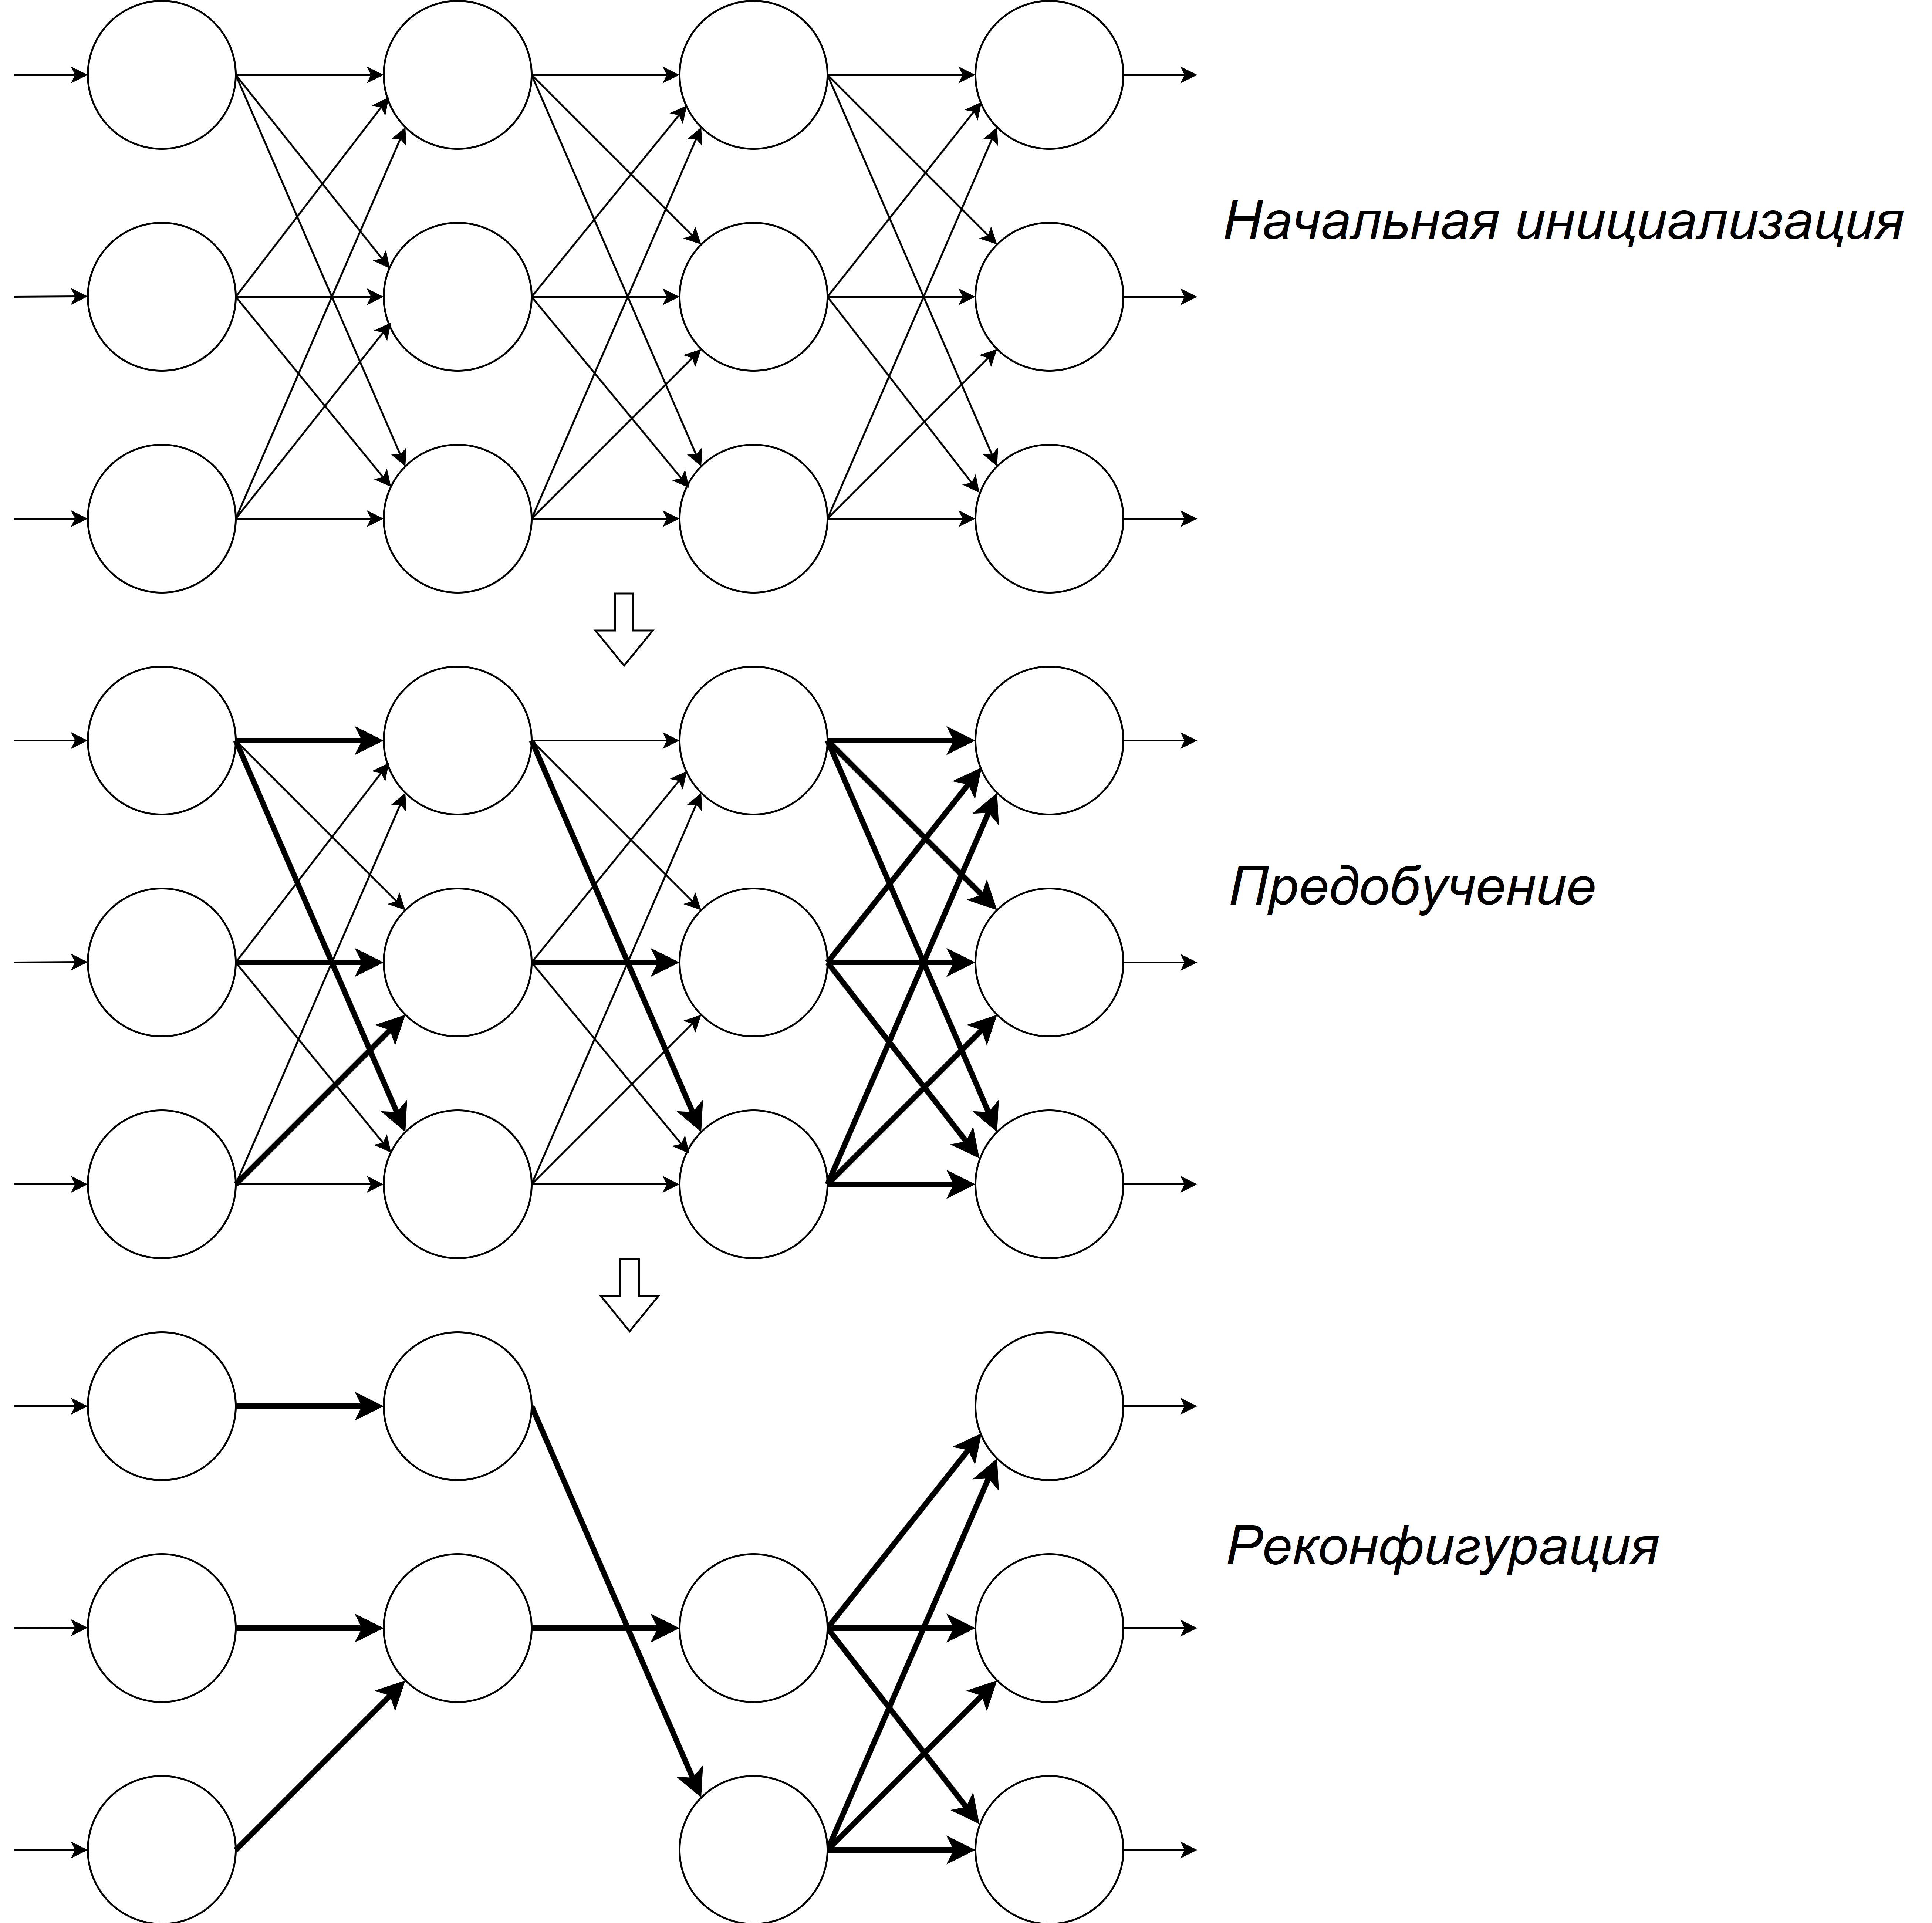
\includegraphics[width=0.7\textwidth]{man-source/images/ch2/pic2-3-1.png}
  \caption{Выполнение редуцирования весовых коэффициентов\\ с архитектурной реконфигурацией НС}
  \label{fig:pic2_3}
\end{figure}

% Этап 3 метода редуцирования может быть представлен следующим алгоритмом:

% \begin{algo}[h]
% 	% \SetAlgoLined
	
% 	\KwIn{\textit{\textbf{x(0)}} -- вектор-образ из обучающей выборки,
% 		$\alpha$ - скорость обучения
% 	}
% 	\KwRes{матрица весовых коэффициентов \textit{\textbf{W}}, вектор порогов нейронов видимого слоя $\textit{\textbf{V}}$, вектор порогов нейронов скрытого слоя $\textit{\textbf{H}}$}
% 	\ForEach{нейрона скрытого слоя $j$}{
% 		Вычислить $P(y_{j}(0)=1|x_{i}(0))$ (для биномиальных нейронов sigmoid($\sum_{i}{w_{ij}x_{i}(0)}+H_j$))\;
% 		Генерировать $y_{j}(0) \in \{0, 1\}$ из $P(y_{j}(0)|x_i(0))$\;
% 	}
% 	\ForEach{нейрона видимого слоя $i$}
% 	{
% 		Вычислить $P(x_{i}(1)=1|y_j(0))$ (для биномиальных нейронов sigmoid($\sum_{j}{w_{ij}y_{j}(0)} + V_i$))\;
% 		Генерировать $x_{i}(1) \in \{0, 1\}$ из $P(x_{i}(1)|y_j(0))$\;
% 	}	
% 	\ForEach{скрытых нейронов $j$}
% 	{
% 		Вычислить $P(y_{j}(1)=1|x_i(1))$ (для биномиальных нейронов sigmoid($\sum_{i}{w_{ij}x_{i}(1)} + H_j$))\;
% 	}
% 	$\textit{\textbf{W}} \leftarrow \textit{\textbf{W}} + \alpha(\textbf{\textit{x(0)}}\textit{\textbf{y(0)}}^T - \textit{\textbf{x(1)}}P(\textit{\textbf{y(1)}}=1|\textit{\textbf{x(1)}})^T)$\;
% 	$\textit{\textbf{V}} \leftarrow \textit{\textbf{V}} + \alpha(\textit{\textbf{x(0)}} - \textit{\textbf{x(1)}})$\;
% 	$\textit{\textbf{H}} \leftarrow \textit{\textbf{H}} + \alpha(\textit{\textbf{y(0)}} - P(\textit{\textbf{y(1)}}=1|\textit{\textbf{x(1)}}))$\;
% %	\While{not at end of this document}{
% %		read current\;
% %		\eIf{understand}{
% %			go to next section\;
% %			current section becomes this one\;
% %		}{
% %		go back to the beginning of current section\;
% %	}
% %}
%     \caption{Процедура обучения RBM}
% 	\label{rbm_learning}
% \end{algo}

% \begin{figure}
% 	\begin{center}
% 		\includegraphics[width=120mm]{reducing_weights.png}
% 		\caption{Метод редуцирования весовых коэффициентов}				
% 		\label{reducing_weigths}
% 	\end{center}
% \end{figure}

% Согласно полученным экспериментальным данным, приведенным в главе \ref{chapt3}, выбор заданного порогового параметра на шаге 2 позволяет значительно упростить архитектуру нейронной сети, сократив количество параметров до 80\% относительно их исходного количества без существенных потерей в обобщающей способности нейронной сети. Данный метод наглядно демонстрирует высокую степень избыточности полносвязных архитектур, используемых для решения задач с небольшими обучающими выборками.

\section{Выводы}
\begin{easylistNum}
    & Предложен альтернативный подход к обучению ограниченной машины Больцмана, базирующийся на идее минимизации суммарной квадратичной ошибки восстановления образов на скрытом и видимом слоях. 
    & Доказана теорема об эквивалентности максимизации функции правдоподобия распределения входных данных \textit{P(x)} и минимизации суммарной квадратичной ошибки восстановления образов на скрытых и видимых слоях в одном и том же пространстве синаптических связей ограниченной машины Больцмана при использовании линейных нейронов.
    & Доказана теорема об эквивалентности максимизации функции правдоподобия распределения входных данных \textit{P(x)} минимизации кросс-энтропийной целевой функции $CE_s(k)$ в одном и том же пространстве синаптических весов ограниченной машины Больцмана (случаи CD-1 и CD-k).
    & Сформулирована обобщающая теорема об эквивалентности максимизации функции правдоподобия распределения входных данных P(x), минимизации кросс-энтропийной функции, минимизации суммарной квадратичной ошибки (специальный случай) в одном и том же пространстве синаптических весов ограниченной машины Больцмана.
    & Приведены правила обучения для различных случаев линейной и нелинейной машины Больцмана (RBM).
    & Приведены правила для обучения сверточных слоев ГНС с использованием модели CRBM.
    & Предложен метод редуцирования параметров глубокой полносвязной нейронной сети, основывающийся на использовании процедуры неконтролируемого предобучения слоев.
\end{easylistNum}
